\documentclass[twoside,12pt]{article}

\usepackage{dsctemplate}
\usepackage[margin=1in]{geometry}
\usepackage{amsmath}
\usepackage{amssymb,amsthm}
\usepackage{fancyhdr}
\usepackage{nicefrac}
\usepackage{minted}
\usetikzlibrary{quotes,angles,positioning,arrows.meta}
\usetikzlibrary{calc}
\usepackage{enumitem}
\usepackage{fancyvrb}
\usepackage{dirtytalk}
\usepackage{comment}

\DefineVerbatimEnvironment{verbatim}{Verbatim}{xleftmargin=.5in}

% \renewcommand{\rmdefault}{phv} % Arial
% \renewcommand{\sfdefault}{phv} % Arial

% configuration
% ------------------------------------------------------------------------------

% control whether solutions are shown or hidden
% \showsolntrue

% page headers only on odd pages
\pagestyle{fancy}
\fancyhead{}
\fancyhead[RO]{PID: \rule{3in}{.5pt}}
\renewcommand{\headrulewidth}{0pt}

% ------------------------------------------------------------------------------

\begin{document}


\thispagestyle{empty}

\vspace{-.5in}

\pstitle{%
    Final Exam%
}{DSC 10, Spring 2023}

\vspace{-.3in}

\hline

\vspace{.1in}

\textbf{Instructions:}
    \begin{itemize}
        \item This exam consists of 11 questions, worth a total of 120 points.
        \item Write your PID in the top right corner of each page in the space provided.
        \item Please write \textbf{clearly} in the provided answer boxes; we will not grade work that appears elsewhere. Completely fill in bubbles and square boxes; if we cannot tell which option(s) you selected, you may lose points.
        
            \bubble{A bubble means that you should only \textbf{select one choice}.}
            
            \squarebubble{A square box means you should \textbf{select all that apply}.}
            
        \item You may refer to the Reference Sheet that was provided to you. Other than that, you may not refer to any other resources or technology during the exam (including calculators).
    \end{itemize}
    
\vspace{.1in}

\hline

\vspace{.1in}

\begin{tabular}{rl}
    Full Name: & \inlineresponsebox[4in]{Solutions}\\
    PID: & \inlineresponsebox[4in]{A12345678}\vspace{.1in}\\
    Lecture Section: & \bubble{A (Sitting in Center 109)} \bubble{B (Sitting in Center 105)} \vspace{.1in} \\ 
%    Initials of student to your left: & \inlineresponsebox[1.5in]{}\\ Initials of student to your right: & \inlineresponsebox[1.5in]{} 
    Seat you are in: & \inlineresponsebox[4in]{}\
\end{tabular}

\vspace{.25in}

\noindent By signing below, you are agreeing that you will behave honestly and fairly during
and after this exam.

\begin{tabular}{rl}
    \: \: \: \: \: Signature: & \inlineresponsebox[4in]{}\\
\end{tabular}

\vfill

\begin{center}
{\huge Version A} \vspace{.2in}

    Please do not open your exam until instructed to do so.
\end{center}

\vspace{1em}

\newpage

\noindent \textbf{Welcome to the Final Exam for DSC 10 in Spring 2023!}

\vspace{.1in}

\noindent You may have noticed that San Diego was quite cloudy in May. In fact, according to the National Weather Service, San Diego was the single cloudiest city in the contiguous United States in May, with clouds covering the sky 82\% of the time. (Only a remote town in Alaska was cloudier!)

\vspace{.1in}

\noindent In this exam, we will work with the DataFrame \texttt{sun}, which describes the number of sunshine hours per month in various cities around the world. Each number in \texttt{sun} is an average across multiple years and multiple sensors.

\vspace{.1in}

\noindent The first 2 columns in \texttt{sun} are \texttt{"Country"} and \texttt{"City"}, which are strings describing a particular city. The next 12 columns are \texttt{"Jan"}, \texttt{"Feb"}, \texttt{"Mar"}, ..., \texttt{"Dec"}, which describe the number of sunshine hours seen each month. The last column, \texttt{"Year"}, is the sum of the month-specific columns.

\vspace{.1in}

\noindent The first few rows of \texttt{sun} are shown below, though \texttt{sun} has many more rows than are shown below.

\begin{center}
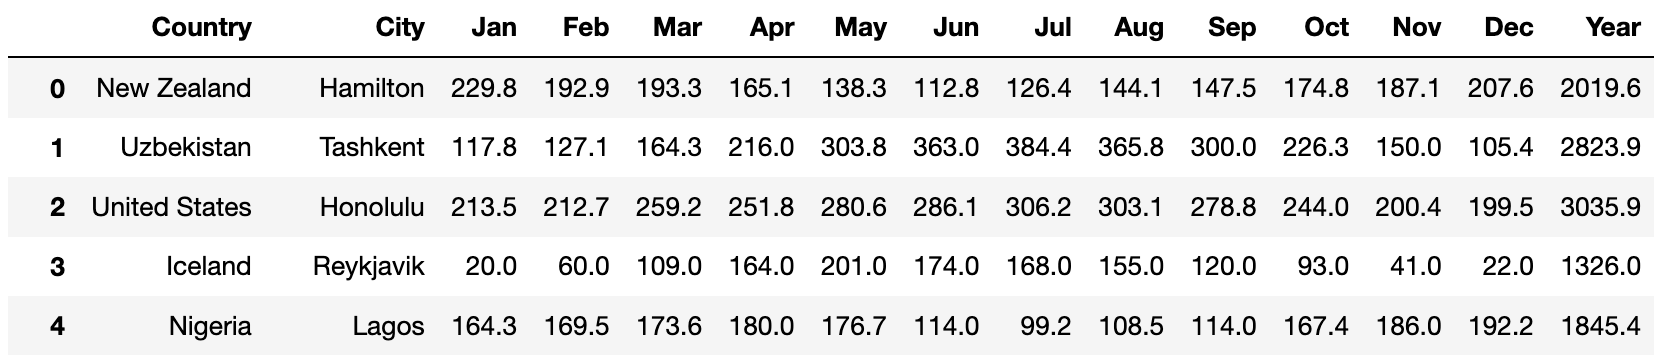
\includegraphics[width=\textwidth]{final_images/sun.png}
\end{center}

\noindent For instance, we see that Tashkent, Uzbekistan sees 164.3 sunshine hours in March.

\vspace{.1in}

\noindent \textbf{Throughout the exam}, assume that we have already run \texttt{import babypandas as bpd} and \texttt{import numpy as np}.

\vspace{.5in}

\noindent \textbf{Advice: Read through all of the questions on the exam first before starting. The questions are not sorted by difficulty!}


\newpage


\begin{probset}

